\documentclass[10pt,onecolumn]{article}
\usepackage[utf8]{inputenc}
 
\pagenumbering{arabic}
%\usepackage{KJN}
\usepackage{siunitx}
\usepackage{graphicx}
\usepackage{placeins}
\usepackage{adjustbox}
\usepackage{fancyvrb}
\usepackage{tablefootnote}
\usepackage{mathtools}
\usepackage[margin=0.75in]{geometry} %This is for all the margins
\usepackage{amsmath}
\usepackage{algorithm}
\usepackage[noend]{algpseudocode}

\def\@maketitle{%
  \null
  \vskip 2em%
  \begin{center}%
  \let \footnote \thanks
    {\LARGE \@title \par}%
    \vskip 1.5em%
    {\large
      \lineskip .5em%
      \begin{tabular}[t]{c}% <------
        \@author%            <------ Authors
      \end{tabular}\par}%    <------
    \vskip 1em%
  %  {\large \@date}%
  \end{center}%
  \par
  \vskip 1.5em}

\date{10/04/2018}

\title{\vspace{-2.2cm} \textbf{ELEN4020: Data Intensive Computing \\ Laboratory Exercise 3}}
\author{\begin{tabular}{ll}
  Kavilan Nair & 1076342 \\
  Christopher Maree & 1101946 \\
  Iordan Tchaparov &  1068874 \\
  Laura West & 1084327\\
\end{tabular}
 }


\begin{document}
%\centering
%\title{\Large{\textbf{ ELEN4020: Data Intensive Computing \\ Laboratory Exercise 1: K-Dimensional Integer Arrays }}}
%\author{Kavilan Nair - 1076342 \\ Iordan Tchaparov - 1068874\\ Christopher Maree - 1101946  \\ Laura West - 1084327 \\ 22/02/2018}



\maketitle
\thispagestyle{empty}\pagestyle{empty}
\vspace{-8mm}

\section*{Matrix Multiplication using Map Reduce}
\noindent In this lab, two different algorithms that performed matrix multiplication through Map Reduce techniques were implemented and tested against each other using different inputs. The algorithms are outlined in this report and compared to find the most time efficient algorithm to process large matrices. The pseudo code for each algorithm is given in the appendix.

\section{Map Reduce}
Map Reduce is a programming model used for the processing of large data sets through distribution on a number of computer clusters. It makes use of parallelized algorithms to process the distributed pieces of data at a much faster rate than if it was done in serial. The Map Reduce model is composed of two stages: the map stage and the reduce stage. The map stage involves taking an input data set and grouping it in a specific way, assigning it a key which can be used to identify the data. The map stage produces tuples consisting of a $key\backslash$value pair. The reduce stage involves taking in the results of the map stage and grouping the $key\backslash$value tuples together based on key values. This grouping allows efficient processing of the mapped data as similar data is grouped together, making it much easier to do manipulations without the need for traditional search and sort algorithms, which would take too much time when applied to large data sets.

\section{Matrix Multiplication}
Matrix multiplication can only occur once matrices fulfill the condition whereby the number of columns of the one matrix must equal to the number of rows of the other matrix. The matrices are input through the use of the Matrix-Market format which specifies the x position, y position and value of the element as one line in a text file, separated by a space. The first line of the text file has the dimensions of the matrix. An illustration of matrix multiplication using this input format with Map Reduce can be found in Figure \ref{diagram} below.

\begin{figure}[h!]
\centering
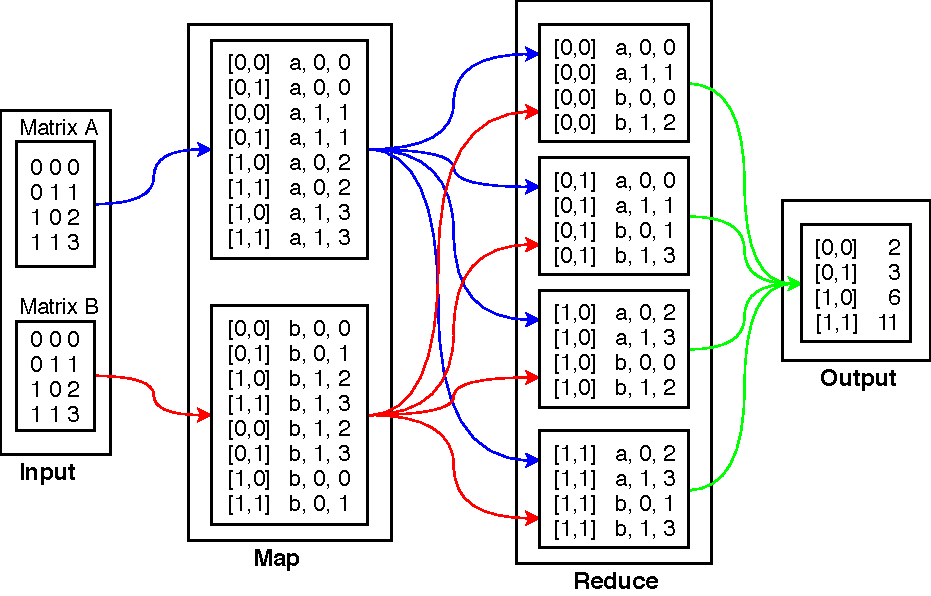
\includegraphics[width=0.8\columnwidth,height=66mm]{diagram.pdf}
\centering
\caption{The process of mapping and reducing for matrix multiplication.}
\label{diagram}
\end{figure}

\noindent The matrices used in Figure \ref{diagram} have dimensions of 2x2 and their elements have values of 0, 1, 2 and 3. In the map stage, the input matrix has its elements mapped to a specific key that is based on the co-ordinates of the element in the matrix, indexed from 0. This key can then be used to identify which $key\backslash$value pairs belong in what position in the output matrix. In the reduce stage, the tuples are grouped together for processing, in this case the multiplication of values and the addition of the results. These are then output together as the resulting matrix.

\section{Implemented Algorithms}
The algorithms were coded in python2.7 and made use of MrJob as the Map Reduce framework. Both of these algorithms were naive iterations of the input data but using a different number of map and reduce functions.

\subsection{Algorithm A}
This algorithm makes use of one map and reduce function in the Map Reduce job and needed processing prior to the execution of the job. This preprocessing was required to get the dimensions of the input matrices to verify if they are of the correct size to allow matrix multiplication and because the i, j and k values were needed for the mapper stage of the algorithm (i and j are the number of rows and columns of matrix A while j and k are the number of rows and columns of matrix B). The pseudo code for this algorithm can be found in the appendix. A criticism of this algorithm is that in the reduce stage, two temporary vectors of size j, filled with zeros, are created to store the elements of matrix A and B that need to be multiplied. These can be very large, at times only storing one value and thus wasting space. The entire vectors are also traversed and the values are multiplied, which can take more time than required if only one position of the vector is filled. This makes the algorithm quite inefficient.

\subsection{Algorithm B}
This algorithm makes use of two map and two reduce functions in the Map Reduce job. It requires no preprocessing as the first map function does not need to know the dimensions of either input matrix. The function produces $key\backslash$value tuple pairs based on a element's x and y position. The first reduce function groups the values based on the keys and then does multiplication of the elements with the same keys. These are saved in a different $key\backslash$value tuple pair. The second map function creates new $key\backslash$value tuple pairs based on the co-ordinates of elements that need to be summed and the second reduce function does the summation. This results in the output matrix. This algorithm uses a dynamic vector for store, that is one that grows in size as it is needed, which makes it much more space efficient than Algorithm A. 

\subsection{Results}
The two algorithms were tested against randomly generated dense matrices with element values being randomly chosen from between 1 to 10. The input matrices had the same sizes (both were of dimensions NxN). The algorithms were run on the following specifications: i5-5200U CPU @ 2.20GHz, 6GB RAM and 1 TB HDD. Table \ref{results} shows the timed results of the algorithms and Figure \ref{graph} shows a graphical representation. 

\begin{table}[h!]
\centering
\caption{Time for NxN matrix multiplication}
\label{results}
\begin{tabular}{|c|l|l|lll|l|l|l|}
\cline{1-3} \cline{7-9}
\textbf{N} & \multicolumn{1}{c|}{\textbf{\begin{tabular}[c]{@{}c@{}}Algorithm A\\ (seconds)\end{tabular}}} & \multicolumn{1}{c|}{\textbf{\begin{tabular}[c]{@{}c@{}}Algorithm B\\ (seconds)\end{tabular}}} &  &  &  & \multicolumn{1}{c|}{\textbf{N}} & \multicolumn{1}{c|}{\textbf{\begin{tabular}[c]{@{}c@{}}Algorithm A\\ (seconds)\end{tabular}}} & \multicolumn{1}{c|}{\textbf{\begin{tabular}[c]{@{}c@{}}Algorithm B\\ (seconds)\end{tabular}}} \\ \cline{1-3} \cline{7-9} 
10         & 0.138416051865                                                                                & 0.240471839905                                                                                &  &  &  & 90                              & 19.7089319229                                                                                 & 16.409126997                                                                                  \\ \cline{1-3} \cline{7-9} 
20         & 0.334219932556                                                                                & 0.436453819275                                                                                &  &  &  & 100                             & 28.2070500851                                                                                 & 22.6466631889                                                                                 \\ \cline{1-3} \cline{7-9} 
30         & 0.855119943619                                                                                & 0.894391775131                                                                                &  &  &  & 125                             & 53.5431759357                                                                                 & 43.0144729614                                                                                 \\ \cline{1-3} \cline{7-9} 
40         & 1.87035703659                                                                                 & 1.72397303581                                                                                 &  &  &  & 150                             & 99.0562970638                                                                                 & 77.0159590244                                                                                 \\ \cline{1-3} \cline{7-9} 
50         & 3.50974607468                                                                                 & 3.16782402992                                                                                 &  &  &  & 175                             & 151.549255848                                                                                 & 123.77800107                                                                                  \\ \cline{1-3} \cline{7-9} 
60         & 6.11380505562                                                                                 & 5.02749991417                                                                                 &  &  &  & 200                             & 226.672954082                                                                                 & 183.890969038                                                                                 \\ \cline{1-3} \cline{7-9} 
70         & 9.92042779922                                                                                 & 8.07861804962                                                                                 &  &  &  & 225                             & 320.148020029                                                                                 & 258.141698122                                                                                 \\ \cline{1-3} \cline{7-9} 
80         & 14.2559621334                                                                                 & 11.5406229496                                                                                 &  &  &  & 250                             & 471.931934118                                                                                 & 343.556027889                                                                                 \\ \cline{1-3} \cline{7-9} 
\end{tabular}
\end{table}

\newpage

\begin{figure}[h!]
\centering
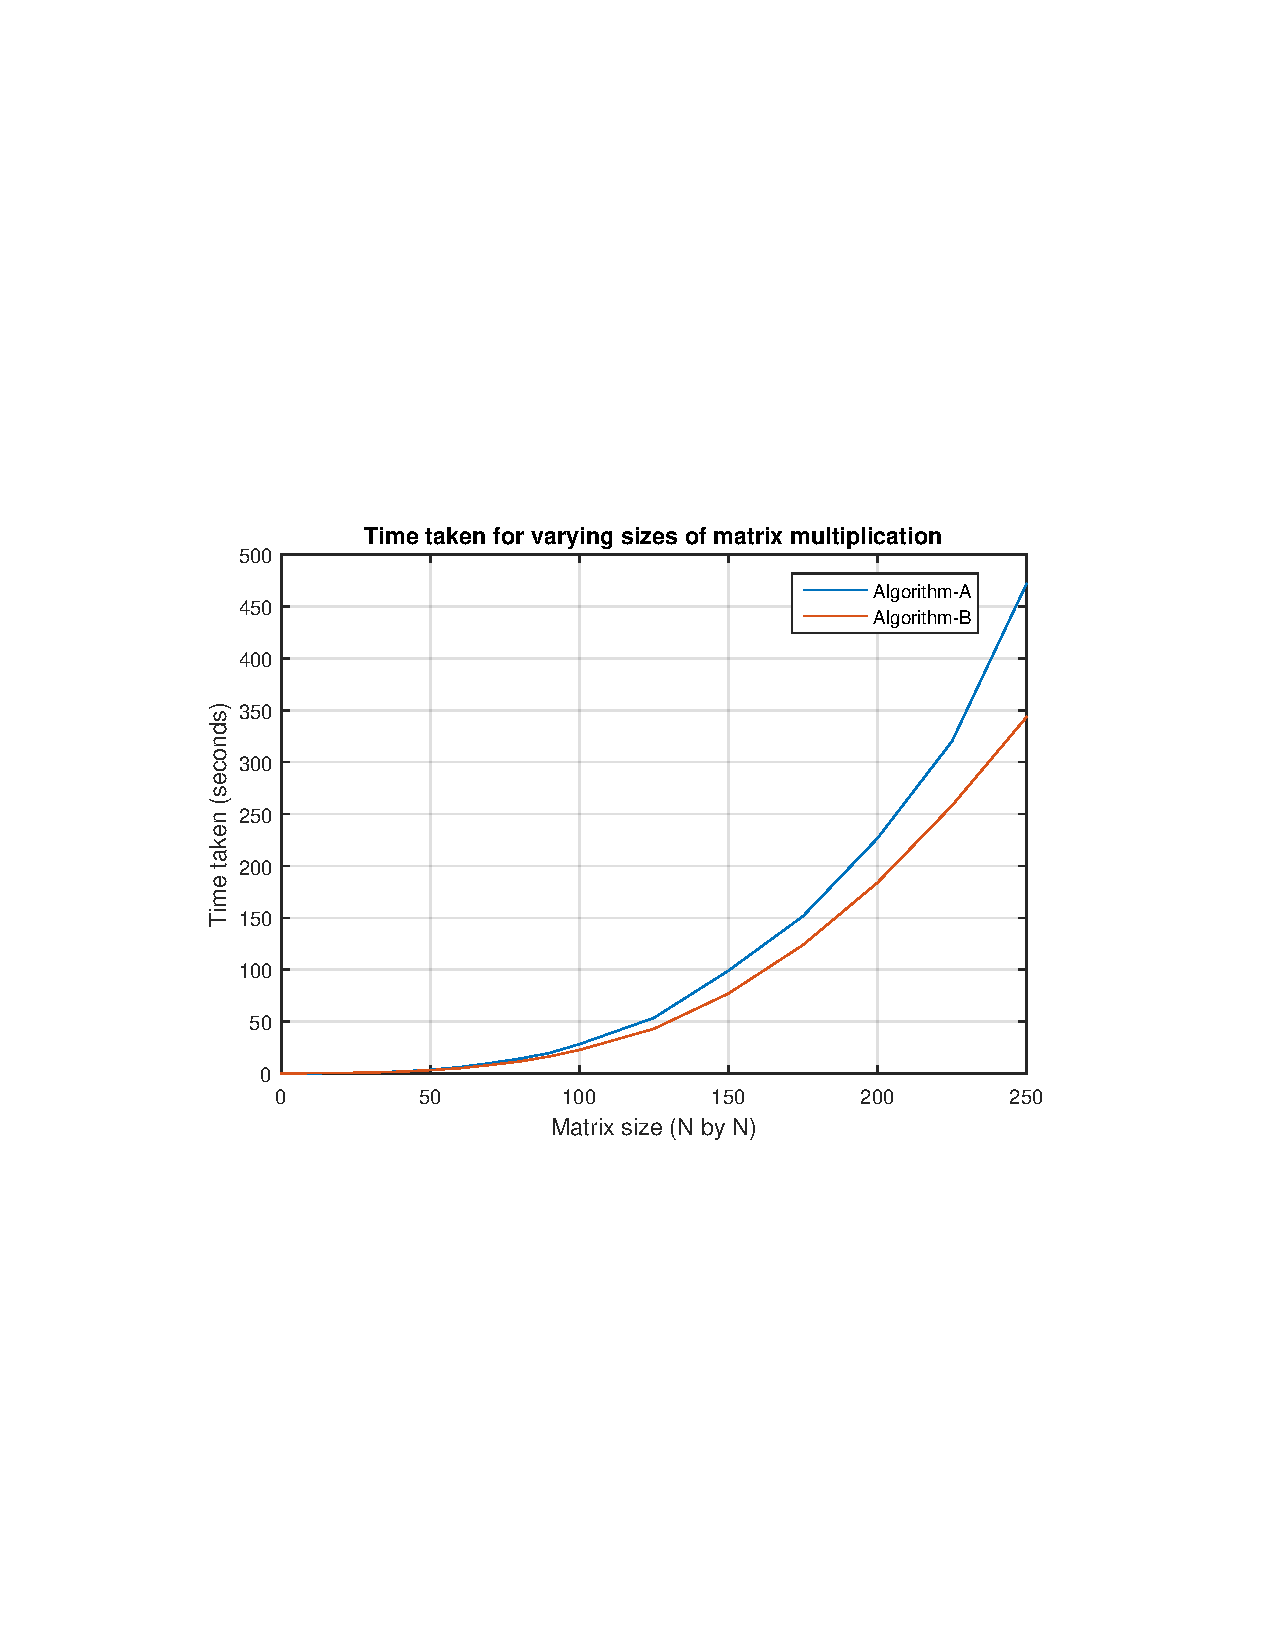
\includegraphics[width=\columnwidth,height=100mm]{graph.pdf}
\centering
\caption{The time taken for matrix multiplication.}
\label{graph}
\end{figure}

\noindent The algorithms were also tested with sparse given inputs. Table \ref{otoo} shows the time it took for these different input files. The second set of input files could not be computed as the computer did not have enough memory to perform the matrix multiplication.

\begin{table}[h!]
\centering
\caption{Time taken for the provided input}
\label{otoo}
\begin{tabular}{|c|l|l|l|}
\hline
\textbf{Name of input files} & \multicolumn{1}{c|}{\textbf{\begin{tabular}[c]{@{}c@{}}Size of matrix\\ multiplication\end{tabular}}} & \multicolumn{1}{c|}{\textbf{\begin{tabular}[c]{@{}c@{}}Algorithm A\\ (seconds)\end{tabular}}} & \multicolumn{1}{c|}{\textbf{\begin{tabular}[c]{@{}c@{}}Algorithm B\\ (seconds)\end{tabular}}} \\ \hline
outA1.list \& outB1.list     & (100 x 100) X (100 x 100)                                                                             & 22.431841135                                                                                  & 14.8576881886                                                                                 \\ \hline
outA2.list \& outB2.list     & (1000 x 500) X (500 x 1000)                                                                           & Cannot compute                                                                                & Cannot compute                                                                                \\ \hline
outA3.list \& outB3.list     & (1000 x 500) X (500 X 1)                                                                              & 11.7946779728                                                                                 & 12.9348580837                                                                                 \\ \hline
\end{tabular}
\end{table}

\section{Unweighted directed graph}
Graphs can be represented through the use of a matrix. The matrices would have elements with values of 1 to indicate connections between nodes and elements with values of 0 to indicate no connection. The degree of the matrix ($A^{n}$ where n is the degree) is the number of paths from which the row node can go to the column node in n steps. As the nodes which are connected by paths of length 3 are wanted, the matrix has to be multiplied by itself and then this result multiplied again by the original matrix to get $A^{3}$. Summing all elements of this matrix will give the number of pairs of nodes that are connected by a path length of 3. This has applications in transport and computer networks, where specific paths can be found alongside other important statistical data. Table \ref{path} below shows the output of the given input file, which was computed on Algorithm B. 

\begin{table}[h!]
\centering
\caption{Results of the input file {\it outNetwork.list}}
\label{path}
\begin{tabular}{|c|c|c|c|c|}
\hline
\textbf{\begin{tabular}[c]{@{}c@{}}Matrix\\ Size\end{tabular}} & \textbf{\begin{tabular}[c]{@{}c@{}}Number of \\ $A^{1}$ Elements\end{tabular}} & \textbf{\begin{tabular}[c]{@{}c@{}}Number of\\  $A^{2}$ Elements\end{tabular}} & \textbf{\begin{tabular}[c]{@{}c@{}}Number of\\  $A^{3}$ Elements\end{tabular}} & \textbf{\begin{tabular}[c]{@{}c@{}}Number of paths\\ of length 3\end{tabular}} \\ \hline
500 x 500                                                      & 31028                                                                                      & 117181                                                                                     & 118604                                                                                     & 39784709                                                                       \\ \hline
\end{tabular}
\end{table}


\section{Conclusion}
This report investigated two Map Reduce algorithm implementations for matrix multiplication. From the results, Algorithm B was discovered to be more efficient and should be used over Algorithm A as it requires less time and space for its processing. The algorithm also requires no preprocessing as it does not use the dimensions of the matrices for its $key\backslash$value tuple pairs. This algorithm was applied to a graph that is represented by a Matrix-Market format and found the nodes which are connected by paths of length 3.

\newpage
\section*{Appendix - Pseudo Code}
\makeatletter
\def\BState{\State\hskip-\ALG@thistlm}
\makeatother
\begin{algorithm}
\caption{One step naive iteration}\label{1step}
\begin{algorithmic}[1]
\State get number of rows and columns in matrix 1 \\
get number of rows and columns in matrix 2 \\
\If {$\textit{number of columns in matrix 1 are not equal to number of rows in matrix 2}$} 
\State Produce error message
\State \textbf{close}
\EndIf \\
check if number of columns in matrix 1 are equal to number of rows in matrix 2.\\ Allocate number of columns in matrix 1 to k
\Procedure{MAP}{} \\
\State get row number (i), column number (j) and element value
\If {$\textit{value is from Matrix 1}$} 
\For {$\textit{column in Matrix 1 from 0 to k-1}$} 
\State yield \textit{(key, value)} pairs as \textit{(i,column), ('Matrix-identifier-1', j, $element value$)} \\
\EndFor
\EndIf
\If {$\textit{values is from Matrix 2}$} 
\For {$\textit{row in matrix 2 from 0 to k-1}$} 
\State yield \textit{(key, value)} pairs as \textit{(row,j), ('Matrix-identifier-2', i, $element value$)} \\
\EndFor
\EndIf
\EndProcedure
\Procedure{REDUCE}{} \\
create empty answer matrix \\
create two empty row vectors of size k, one for matrix 1 and one for matrix 2
\For {$\textit{x in value of the (key, value) pair}$}
\If {$\textit{value is from matrix 1}$}
\State position = x[1]
\State matrix 1 row vector at position = element value
\Else 
\State position = x[1]
\State matrix 2 row vector at position = element value
\EndIf
\EndFor
\For {$\textit{interator from 0 to k-1}$}
\State Append (matrix 1 row vector value[iterator] x matrix 2 row vector value[iterator] ) to answer matrix
\EndFor
yield key, sum of answer matrix values
\EndProcedure
\end{algorithmic}
\end{algorithm}

\newpage

\begin{algorithm}
\caption{Two step naive iteration}\label{2step}
\begin{algorithmic}[1]
\Procedure{MAP1}{} \\
\State get row number (i), column number (j) and value
\If {$\textit{value is from Matrix 1}$} 
\For {$\textit{column in Matrix 1 from 0 to k-1}$} 
\State yield \textit{(key, value)} pairs as \textit{ j, ('Matrix-identifier-1', i, $value$)} \\
\EndFor
\EndIf
\If {$\textit{values is from Matrix 2}$} 
\For {$\textit{row in matrix 2 from 0 to k-1}$} 
\State yield \textit{(key, value)} pairs as \textit{i, ('Matrix-identifier-2', j, $value$)} \\
\EndFor
\EndIf
\EndProcedure
\Procedure{REDUCE1}{} \\
create two empty row vectors, one for matrix 1 and one for matrix 2
\For {$\textit{x in value of the (key, value) pair}$}
\If {$\textit{value is from matrix 1}$}
\State append x to matrix 1 row vector
\Else 
\State append x to matrix 2 row vector
\EndIf
\EndFor
\For {x in matrix 1 row vector}
\For {y in matrix 2 row vector}
 yield key, (x[1], y[1], x[2]*y[2])
\EndFor
\EndFor
\EndProcedure
\Procedure{MAP2}{}\\
from \textit{(key, value)} pair: \\
yield (value[0], value[1]), value[2]
\EndProcedure
\Procedure{REDUCE2}{}\\
yield key, sum(value)
\EndProcedure
\end{algorithmic}
\end{algorithm}


\end{document}